\documentclass[tikz,border=5pt]{standalone}
\usepackage{tikz}
\usetikzlibrary{arrows.meta}
\begin{document}
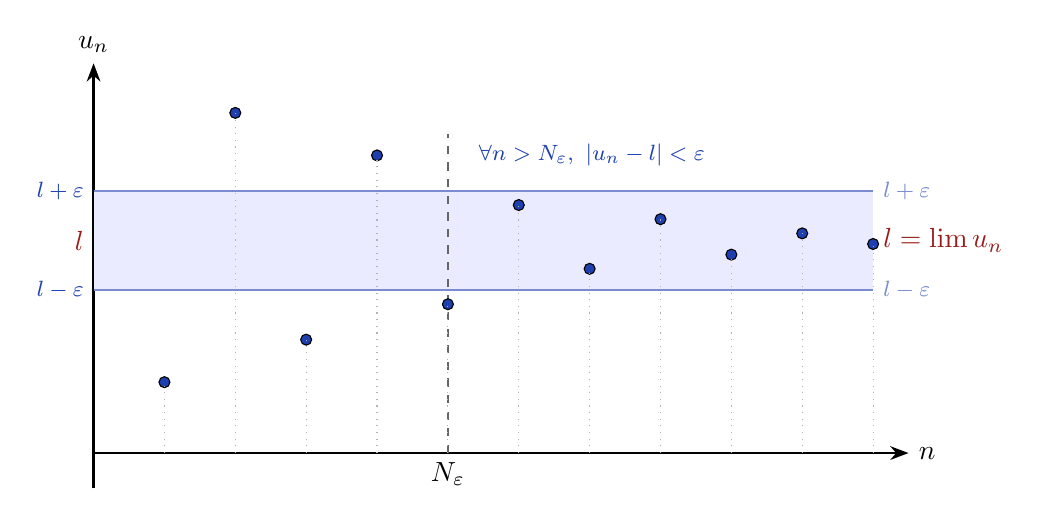
\begin{tikzpicture}[>=Stealth, scale=0.9]
  \definecolor{setblue}{HTML}{1E40AF}
  \definecolor{accentcrimson}{HTML}{991B1B}

  % Axes
  \draw[thick, ->] (0,0) -- (11.5,0) node[right, font=\sffamily\bfseries] {$n$};
  \draw[thick, ->] (0,-0.5) -- (0,5.5) node[above, font=\sffamily\bfseries] {$u_n$};

  % Limit line l
  \draw[thick, dashed, accentcrimson] (0, 3.0) -- (11.0, 3.0) node[right, font=\sffamily\bfseries] {$l = \lim u_n$};
  \node[left, accentcrimson, font=\sffamily\bfseries] at (0, 3.0) {$l$};

  % Epsilon tube
  \fill[blue!8] (0, 2.3) rectangle (11.0, 3.7);
  \draw[thick, setblue!60] (0, 3.7) -- (11.0, 3.7) node[right, font=\sffamily\footnotesize] {$l + \varepsilon$};
  \draw[thick, setblue!60] (0, 2.3) -- (11.0, 2.3) node[right, font=\sffamily\footnotesize] {$l - \varepsilon$};
  \node[left, setblue, font=\sffamily\footnotesize] at (0, 3.7) {$l+\varepsilon$};
  \node[left, setblue, font=\sffamily\footnotesize] at (0, 2.3) {$l-\varepsilon$};

  % Threshold N_epsilon
  \draw[thick, dashed, black!60] (5.0, 0) -- (5.0, 4.5);
  \node[below, font=\sffamily\bfseries] at (5.0, 0) {$N_\varepsilon$};

  % Sequence points
  \foreach \n/\val in {1/1.0, 2/4.8, 3/1.6, 4/4.2, 5/2.1, 6/3.5, 7/2.6, 8/3.3, 9/2.8, 10/3.1, 11/2.95} {
    \draw[fill=setblue] (\n, \val) circle (2.2pt);
    \draw[dotted, black!30] (\n, 0) -- (\n, \val);
  }

  \node[anchor=west, font=\sffamily\footnotesize, setblue] at (5.3, 4.2) {$\forall n > N_\varepsilon, \ |u_n - l| < \varepsilon$};
\end{tikzpicture}
\end{document}